%/////////////////////////////////////////////////////////%
%		   
% file: 	wt_template.tex
% version:	0.2 
% modified:	2014-12-25
% author:	Tyler Stephen (tstephen@uvic.ca)
% descr:	A document that follows the University of Victoria
%			style guide for work term reports. The letter of
%			transmittal is included from a separately generated
%			pdf.
%
%/////////////////////////////////////////////////////////%
%%% TODO:
% Appendix
%		XXX remove page numbers from ToC 
%		XXX fix last page number of appendix (does not follow Letter - number format)
%		XXX fix blank page workaround for last page number
% XXX Letter of Transmittal
%		XXX import from another file is probably easiest
% Title Page
%		XXX maybe do the same import thing as the letter
%		XXX recreate the approval graphic in situ
%		make the approval box prettier~*~*~ 
%			less top/bottom padding
%			XXX box is longer than pagewidth
%			fields are aligned (table?)
%		anchor the approval box to the bottom
% References
%		XXX learn how they work
%		XXX find out how URLs\webpages are displayed in ieeetr
%			works with @misc entry but it's clunky. Manual entry of \url and
%			does not display last accessed date. May have to install another bib style


%/////////////////////////////////////////////////////////%
%//						PREAMBLE						//%
%/////////////////////////////////////////////////////////%

\documentclass[11pt]{article}

%%%%%%%%%%%%%%%%%%%%%%%
% 	  Packages
%%%%%%%%%%%%%%%%%%%%%%%

%% Fonts and Symbols
%% --------------------------
\usepackage{
			amsmath,			% math operators
			amssymb,			% math symbols
%			amsthm,				% theorem environment
%			soul,				% strike through with \st{}
%			xfrac,				% fancy fractions
			}		

%% Graphics
%% --------------------
\usepackage{
			graphicx,			% allows insertion of images
			subfigure,			% allows subfigures (a), (b), etc.
			}				
\graphicspath{ {graphics/} }	% (graphicx) relative path to graphics folder				
	
%% Tables
%% --------------------------
\usepackage{
			booktabs,			% better tables, discourages vertical rulings		
			multicol,			% allow multi columns	
			}

%% Layout Alteration
%% --------------------------
\usepackage{			
%			caption,			% line breaks in captions with \\
%			changepage,			% change margins for PARTS of pages with (adjustwidth)
%			fancyhdr,			% see config in LAYOUT AND STYLING
			framed,				% nice boxes; used in Supervisor's Approval
%			fullpage,			% set full page margins
			geometry,			% change the margins for specific PAGES
%			lastpage,			% used with (fancyhdr)
%			parskip,			% disable indents
%			pdflscape,			% ???
%			rotating,			% sideways figures
			}
\geometry{						% specify page size options for (geometry)
			a4paper, 			% paper size
%			hmargin=1in,		% horizontal margins
		 }				

%% Units
%% --------------------------
\usepackage{
			siunitx,			% has S (decimal align) column type
			}
\sisetup{input-symbols = {()},  % do not treat "(" and ")" in any special way
         group-digits  = false, % no grouping of digits
%		 load-configurations = abbreviations,
%		 per-mode = symbol,
		 }
		 
%% Misc
%% --------------------------
\usepackage{
			pdfpages,			% import pdfs into this document -- used for the Letter
			url,				% allows urls to be added to document
			}	
			
			 
%%%%%%%%%%%%%%%%%%%%%%%
% Macros and Commands
%%%%%%%%%%%%%%%%%%%%%%%

% scientific notation  use \e{}
\providecommand{\e}[1]{\ensuremath{\times 10^{#1}}}

% override S column type with centered text column
\providecommand{\textcol}[1]{\multicolumn{1}{c}{#1}}

% easy unit spacing in math mode
\providecommand{\units}[1]{\;\text{#1}}

% provides a place to write on documents; like __________________ that
\providecommand{\blankline}{\underline{\hspace{3cm}}}

% Set up page numbering for appendices as (Appendix Letter) - (Page Number)
\providecommand{\StartAppendices}{
    \newpage
    \newcounter{AppendixCounter}	
    \renewcommand{\thepage}{\Alph{AppendixCounter} - \arabic{page}}
}
	
% Manually construct the section title for each appendix and then
% add an entry to the ToC 
\providecommand{\Appendix}[1]{
    \newpage
    \stepcounter{AppendixCounter}
    \setcounter{page}{1}
    \section*{Appendix \Alph{AppendixCounter}\quad #1}
    \addtocontents{toc}{\protect\contentsline{section}%
    	{Appendix \Alph{AppendixCounter}\quad #1}{}}
	% \protect preserves the spacing in the ToC
}


%%%%%%%%%%%%%%%%%%%%%%%
% 	Environments
%%%%%%%%%%%%%%%%%%%%%%%

% Cleans up the nested environments used to create the approval box
% on the title page
\newenvironment{ApprovalBox}
	{ % beginning formatting
		\begin{framed}			
		\begin{scriptsize}
		\begin{flushleft}
		\begin{small}
	}
	{ % end formatting
		\end{small}
		\end{flushleft}
		\end{scriptsize}
		\end{framed}
	}

% Hides the formatting for the summary
\newenvironment{Summary}
	{ % beginning formatting
		% manually add entry to the toc since section*
		% suppresses addition to toc 
		\addcontentsline{toc}{section}{Summary}	
		\topskip0pt				% remove top padding
		\vspace*{\stretch{2}}	% Pad 2/3 of the page length
		\section*{Summary}		% don't append a section number before "Summary"
	}
	{ % end formatting
		\vspace*{\stretch{3}}
	}

% Hides the formatting for the glossary
\newenvironment{Glossary}
	{ 	%beginning formatting
		\addcontentsline{toc}{section}{Glossary}	
 		\section*{Glossary}		
		\begin{description}
	}
	{
		\end{description}
	}

%/////////////////////////////////////////////////////////%
%//						BODY							//%
%/////////////////////////////////////////////////////////%

\begin{document}

%%%%%%%%%%%%%%%%%%%%%%%
% 	  Title Page
%%%%%%%%%%%%%%%%%%%%%%%
\pagenumbering{gobble}		% turn off page numbering
\newgeometry{hmargin=3cm}	% wider margins to accommodate approval box
\begin{center}
University of Victoria\\
Faculty of Engineering\\
Date Work Term Report\\
\vspace{1cm}

{\huge Name of your report}\\
\vspace{1cm}

Employer name \\
Employer address\\
\vspace{1cm}

Your Name\
V00XXXXXX\\
Work Term X\\
Something Engineering\\
yourname@uvic.ca\\
\vspace{0.5cm}

\today \\
\vspace{1cm}

In partial fulfillment of the requirements of the\\
Bachelor of Engineering Degree\\
\vspace{4cm}



\begin{ApprovalBox}
	\textbf{Supervisor's approval: To be completed by the Co-Op Employer} 
	\newline\newline
	I approve the release of this report to the University of Victoria for evaluation purposes only. 
	\newline\newline
	The report is to be considered: \quad $\square${} NOT CONFIDENTIAL \quad $\square${} CONFIDENTIAL
	\newline\newline
	Signature: \blankline{} Position: \blankline{} Date: \blankline{} \newline\newline
	Name (print): \blankline{} E-Mail: \blankline{} Fax \#: \blankline{} 
	\newline\newline
	If a report is deemed CONFIDENTIAL, a non-disclosure form signed by an evaluator will be faxed to the employer. The report will be destroyed following evaluation. If the report is NOT CONFIDENTIAL, it will be returned to the student following evaluation.
\end{ApprovalBox}

\end{center}
\restoregeometry		% back to a4 size

%%%%%%%%%%%%%%%%%%%%%%%
% Letter of Transmittal
%%%%%%%%%%%%%%%%%%%%%%%
\newpage
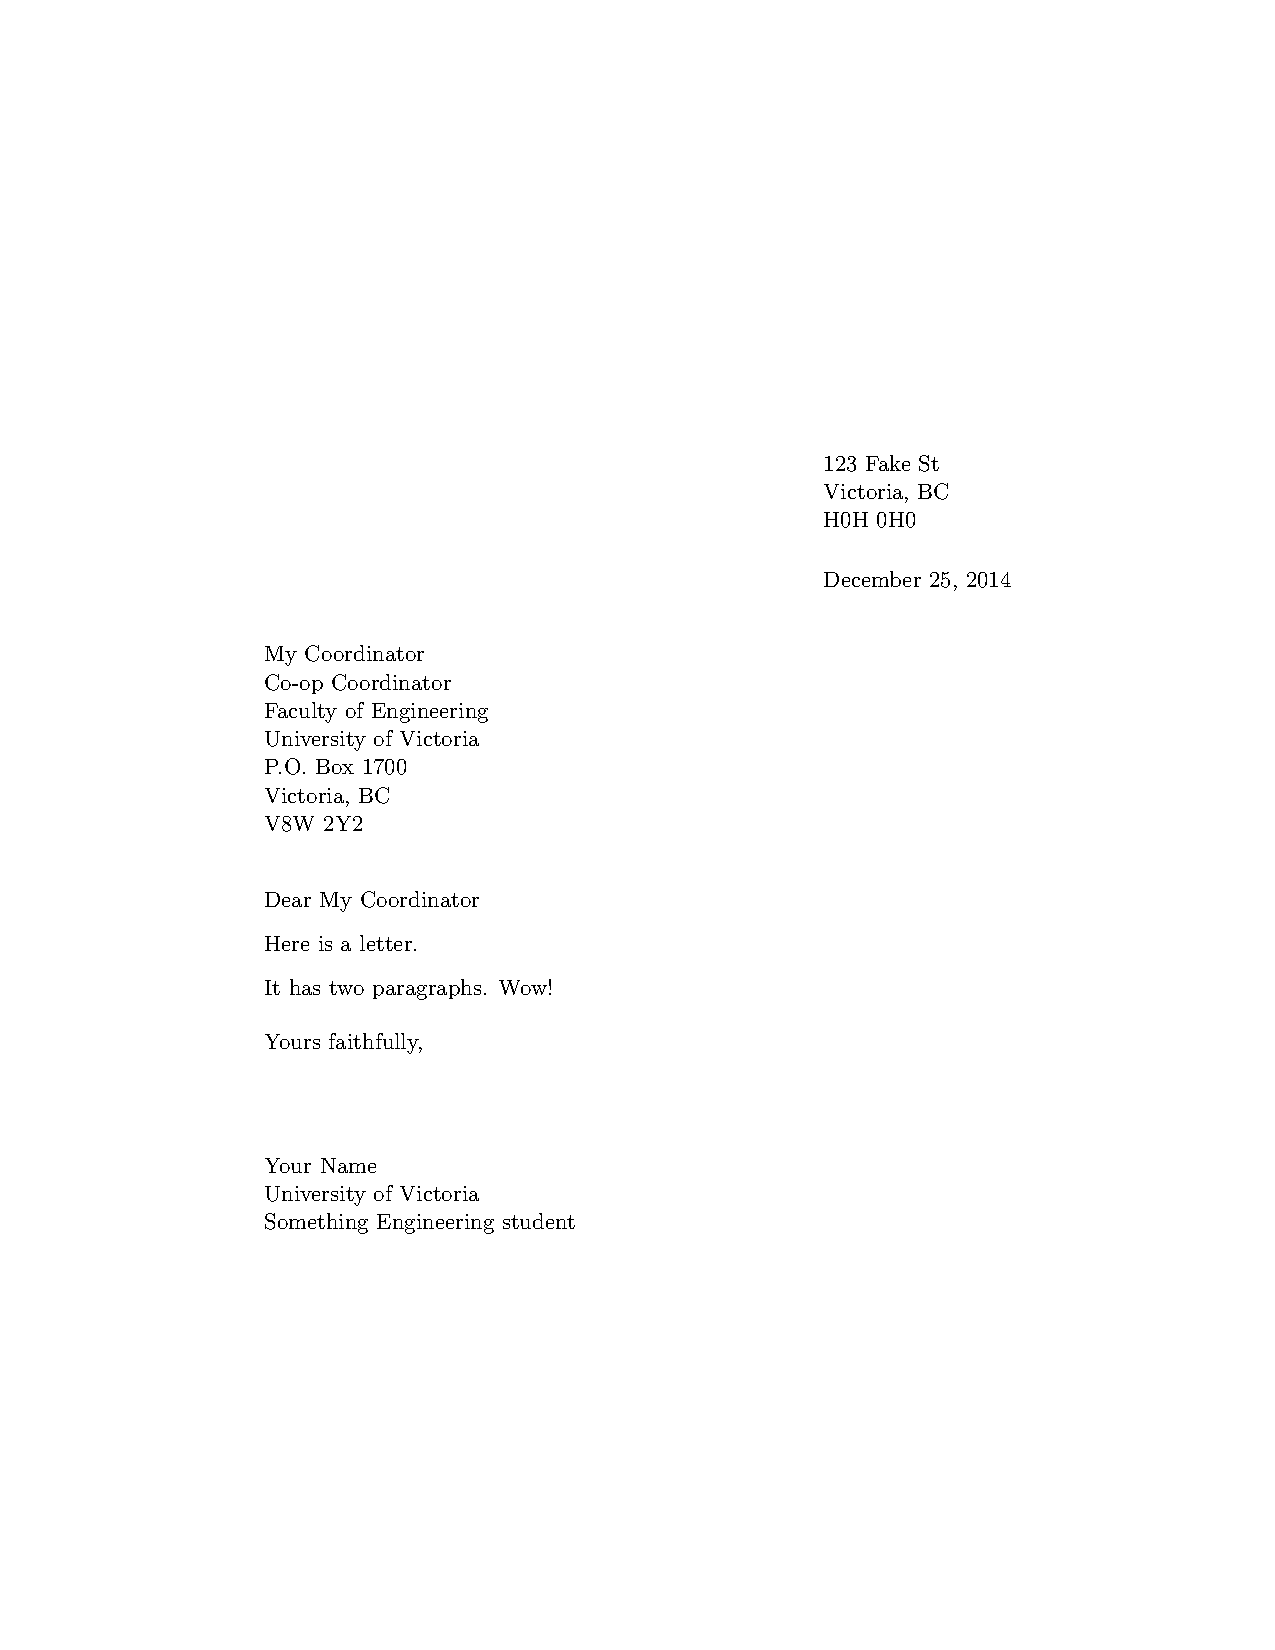
\includepdf{letter/letter_of_transmittal}


%%%%%%%%%%%%%%%%%%%%%%%
%  Tables of Contents
%%%%%%%%%%%%%%%%%%%%%%%
\newpage
\addtocontents{toc}{~\hfill\textbf{Page}\par}	% 'Page' above the page numbers
\tableofcontents

\newpage
\pagenumbering{roman}	% i, ii, iii, ... page numbering
\addcontentsline{toc}{section}{\listfigurename}	% manually add to toc
\addtocontents{lof}{~\hfill\textbf{Page}\par}
\listoffigures

\newpage				% LoF and LoT may be on the same page if they fit
\addcontentsline{toc}{section}{\listtablename}
\addtocontents{lot}{~\hfill\textbf{Page}\par}
\listoftables

%%%%%%%%%%%%%%%%%%%%%%%
% 		Summary
%%%%%%%%%%%%%%%%%%%%%%%
\newpage

\begin{Summary}
The summary is written for the general reader who wishes to be familiar with the content of the report while avoiding details. The summary is a separate report, stating the engineering problem, the approach to the solution, the main conclusions and recommendations. It is written after the main report has been completed. Items in the main report such as tables, figures or sections, are not referred to in the summary. The summary is normally presented centered on its own page, and is less than one page in length.
\end{Summary}

%%%%%%%%%%%%%%%%%%%%%%%
% 		Glossary
%%%%%%%%%%%%%%%%%%%%%%%
\newpage

\begin{Glossary}
	\item[Uvic] University of Victoria
\end{Glossary}

%%%%%%%%%%%%%%%%%%%%%%%
%		Main Body
%%%%%%%%%%%%%%%%%%%%%%%
\newpage
\pagenumbering{arabic}	% 1, 2, 3, ... page numbering

\section{Introduction}
The introduction introduces the report to the reader by:
\begin{itemize}
	\item making a few background statements about the company/organization
	\item introducing the subject to be discussed
	\item mentioning why the subject is important
	\item outlining the content of the rest of the report.
	\item containing sufficient background information for the reader to understand the rest of the
report.
\end{itemize}
Introductions should never be longer than the discussion. If a significant amount of background information is required, some of the material may be included as appendices.
The introductory material may be presented in several sections to cover the scope of the report as well as provide the necessary background information. In the sample Table of Contents, the introductory portion is contained in sections 1 through 4.

\section{Discussion}
The discussion is the foundation of a report. It presents evidence in the form of referenced facts, data, test results, and analysis upon which the conclusions are based. A well-written discussion flows logically from concept to concept to lead the reader to the appropriate conclusions.
The discussion may contain several sections if several concepts are presented. In the sample Table of Contents, the discussion is contained in subsections 5.1 through 5.5.

\section{Conclusion}
Conclusions are the results derived from the evidence provided in the discussion. No new material is presented in the conclusion.
\subsection{sub conclusion}
When presenting more than one conclusion, state the main conclusion first followed by the others in the order of decreasing importance, to ensure the maximum impact on the reader.

\section{Recommendation}
Recommendations are an outline of what further work needs to be done based solidly on the information you previously presented in the report. They have the greatest impact when written using action verbs. Again, do not introduce new material or concepts here\cite{fb}\cite{goog}\cite{uvic}.


%%%%%%%%%%%%%%%%%%%%%%%
% 	  Referrences
%%%%%%%%%%%%%%%%%%%%%%%
\newpage
\addcontentsline{toc}{section}{References}
\bibliographystyle{ieeetr}
\bibliography{wt_template}
% Update entries in bibdesk using texshop to typeset
% typsetting: 1) latex 2) bibdesk 3) latex 4) latex


%%%%%%%%%%%%%%%%%%%%%%%
% 	   Appendices
%%%%%%%%%%%%%%%%%%%%%%%

\StartAppendices

\Appendix{My appendix}
Here is some text for my appendix.

\Appendix{Another appendix}
Here is another appendix. It has multiple pages. Watch the page numbering.
\newpage \null

\Appendix{Last appendix}
This is the last appendix.

\end{document}